\chapter{Kravspecifikation (Alle)}\label{chap:kravspec}

\section{Version}
\begin{table}[h]
	\centering
	\begin{tabularx}{\textwidth - 2cm}{|l|l| l|X|}
	\hline
	Dato	& Version	& Initialer & Ændring	\\ \hline
	8. oktober & 1 & KT	& Første udkast af dokumentet efter review \\ \hline
	19. november & 2 & KR & Glødepære ændret til LED. \\ \hline
	9. december & 3 & KT & Indsat billede af softwaren samt små rettelser. \\ \hline
	15. december & 4 & LS & Små rettelser. Endelig version. \\ \hline
	\end{tabularx}
\end{table}

\section{Systembeskrivelse} \label{Systembeskrivelse}
\subsubsection{PC-software}
Softwaren på brugerens PC er sammen med DE2-boardet grænsefladen til systemet. Når programmet åbnes vil der vises en brugerflade på skærmen, som guider brugeren gennem opsætning og indstilling af systemet. Systemet fortsætter selvom brugerens PC slukkes eller at softwaren lukkes ned, men ønskes interaktion med systemet skal softwaren startes igen. Figur \ref{fig:softwareudkast} viser et udkast af hovedmenuen i userinterfacet.

\begin{figure}[h]
\centering
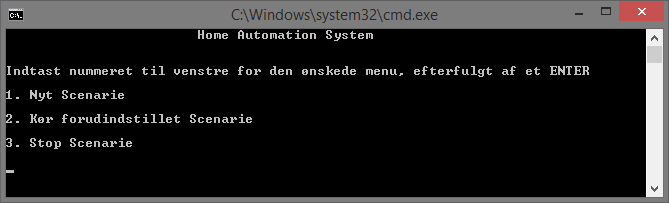
\includegraphics[width=\textwidth - 2.5 cm, clip=true, trim=4 16 50 22]{../Kravspecifikation/swudkast}
\caption{Hovedmenuen for softwaren til PC}
\label{fig:softwareudkast}
\end{figure}

\subsubsection{Scenarier}
Systemet indeholder tre prædefinerede scenarier, som ligger i PC-softwaren. Disse tre scenarier kan ikke ændres og der kan ikke tilføjes flere. Brugeren har derimod mulighed for at oprette et brugerdefineret scenarie, som overføres til transmitter-controlleren og eksisterer så længe det afvikles. Ved afvikling af et nyt scenarie (brugerdefineret eller prædefineret) overskrives det scenarie, som er gemt på transmitter-controlleren. Et scenarie består af op til 20 aktioner, et eksempel på en aktion kunne være ''tænd lampe 1 klokken 12:00'', hvor: ''lampe 1'' er enheden, ''tænd'' er kommandoen og ''12:00'' er tidspunktet. I Tabel \ref{tbl:kommando} nedenfor vises et eksempel på tre aktioner. \hfill

\begin{table}[h]
\centering
\begin{tabularx}{\textwidth - 5cm}{|l|l|X|X|} \hline
Aktionsnummer & Tidspunkt & Enhed & Kommando \\ \hline
1 & 12:00 & Lampe 1 & Tænd \\ \hline
2 & 13:15 & TV & Tænd \\ \hline
3 & 13:30 & TV & Sluk \\ \hline
\end{tabularx}
\label{tbl:kommando}
\caption{Eksempel på scenarie.}
\end{table} \hfill

\subsubsection{Transmitter-controller}
Controlleren modtager de konfigurerede indstillinger fra PC'en og validerer kodelåsen på DE2-boardet, før brugeren kan tilgå PC-softwaren.
Kan koden ikke valideres, sørger transmitter-control-leren for at nægte adgang til systemet.
Når systemet er aktiveret, sørger transmitter-controlleren for at eksekvere det valgte scenarie og afsende kommandoer til de valgte enheders receiver-controllere over elnettet.

\subsubsection{Receiver-controller}
Hver receiver-controller har sit eget enheds-ID, som kun den reagerer på. Ydermere er begge lampe-controllere grupperet under samme huskode, hvor TV-controlleren og radio-controlleren har hver sin huskode. Hver type af receiver-controller understøtter forskellige kommandoer.

\subsubsection{Kodelås DE2}
Kodelåsen bliver indstillet af brugeren ved installation af systemet, denne kan herefter ændres efter brugerens ønske, såfremt den tidligere kode indtastes først.
Kodelåsen kan kun indeholde én kode.

\clearpage
\section{Aktør-kontekst diagram}
\begin{figure}[h]
\centering
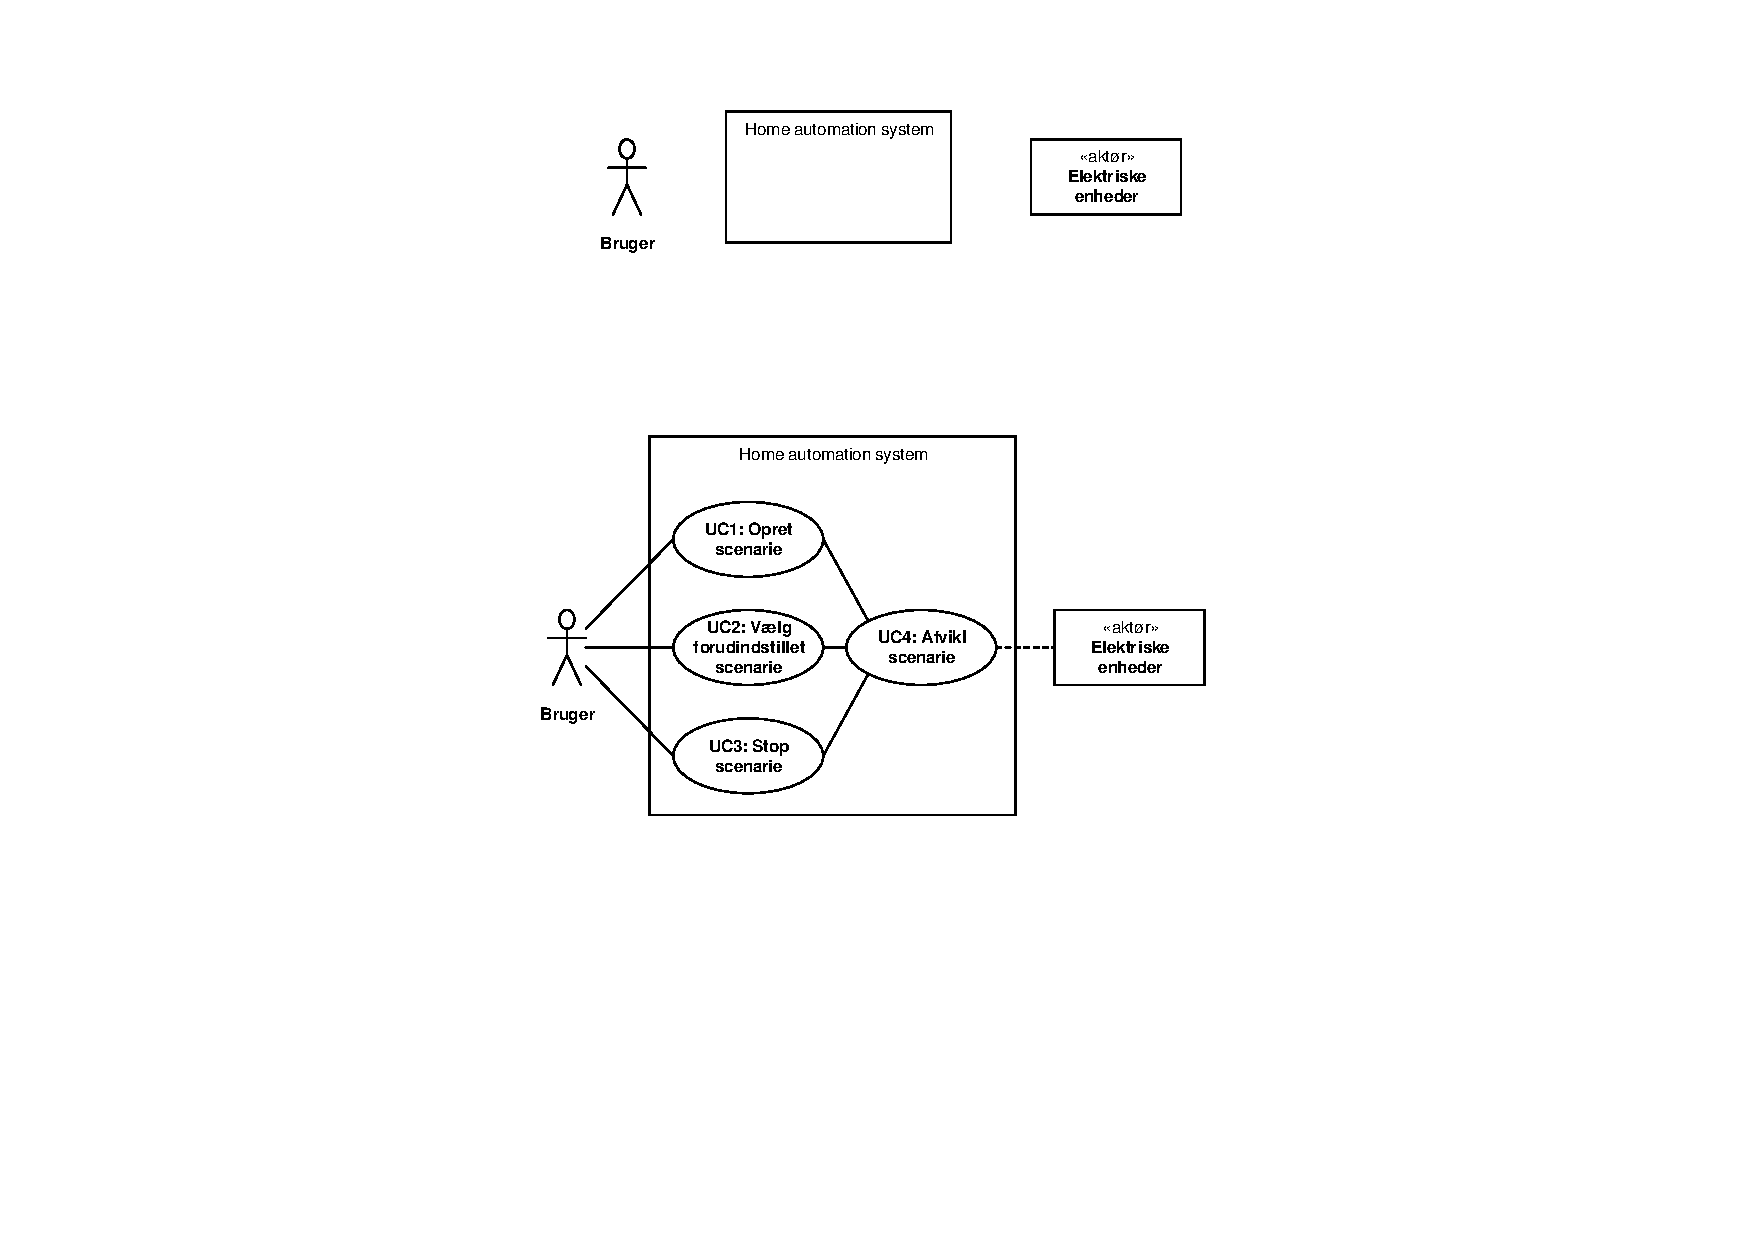
\includegraphics[scale=1,clip=true,trim=250 475 250 50]{../Kravspecifikation/actor.pdf}
\label{fig:actor}
\caption{Aktør-kontekst diagram}
\end{figure}

\subsection{Aktørbeskrivelse}
\subsubsection{Bruger (Primær aktør)}
Brugeren er kunden, som bruger systemet til hverdag. Brugeren ønsker at oprette og afvikle scenarier.

\subsubsection{Elektriske enheder (Sekundær aktør)}
Elektriske enheder er hhv. to lamper, et fjernsyn og en radio, der er tilkoblet systemet.

\section{Use Case diagram}
\begin{figure}[h]
\centering
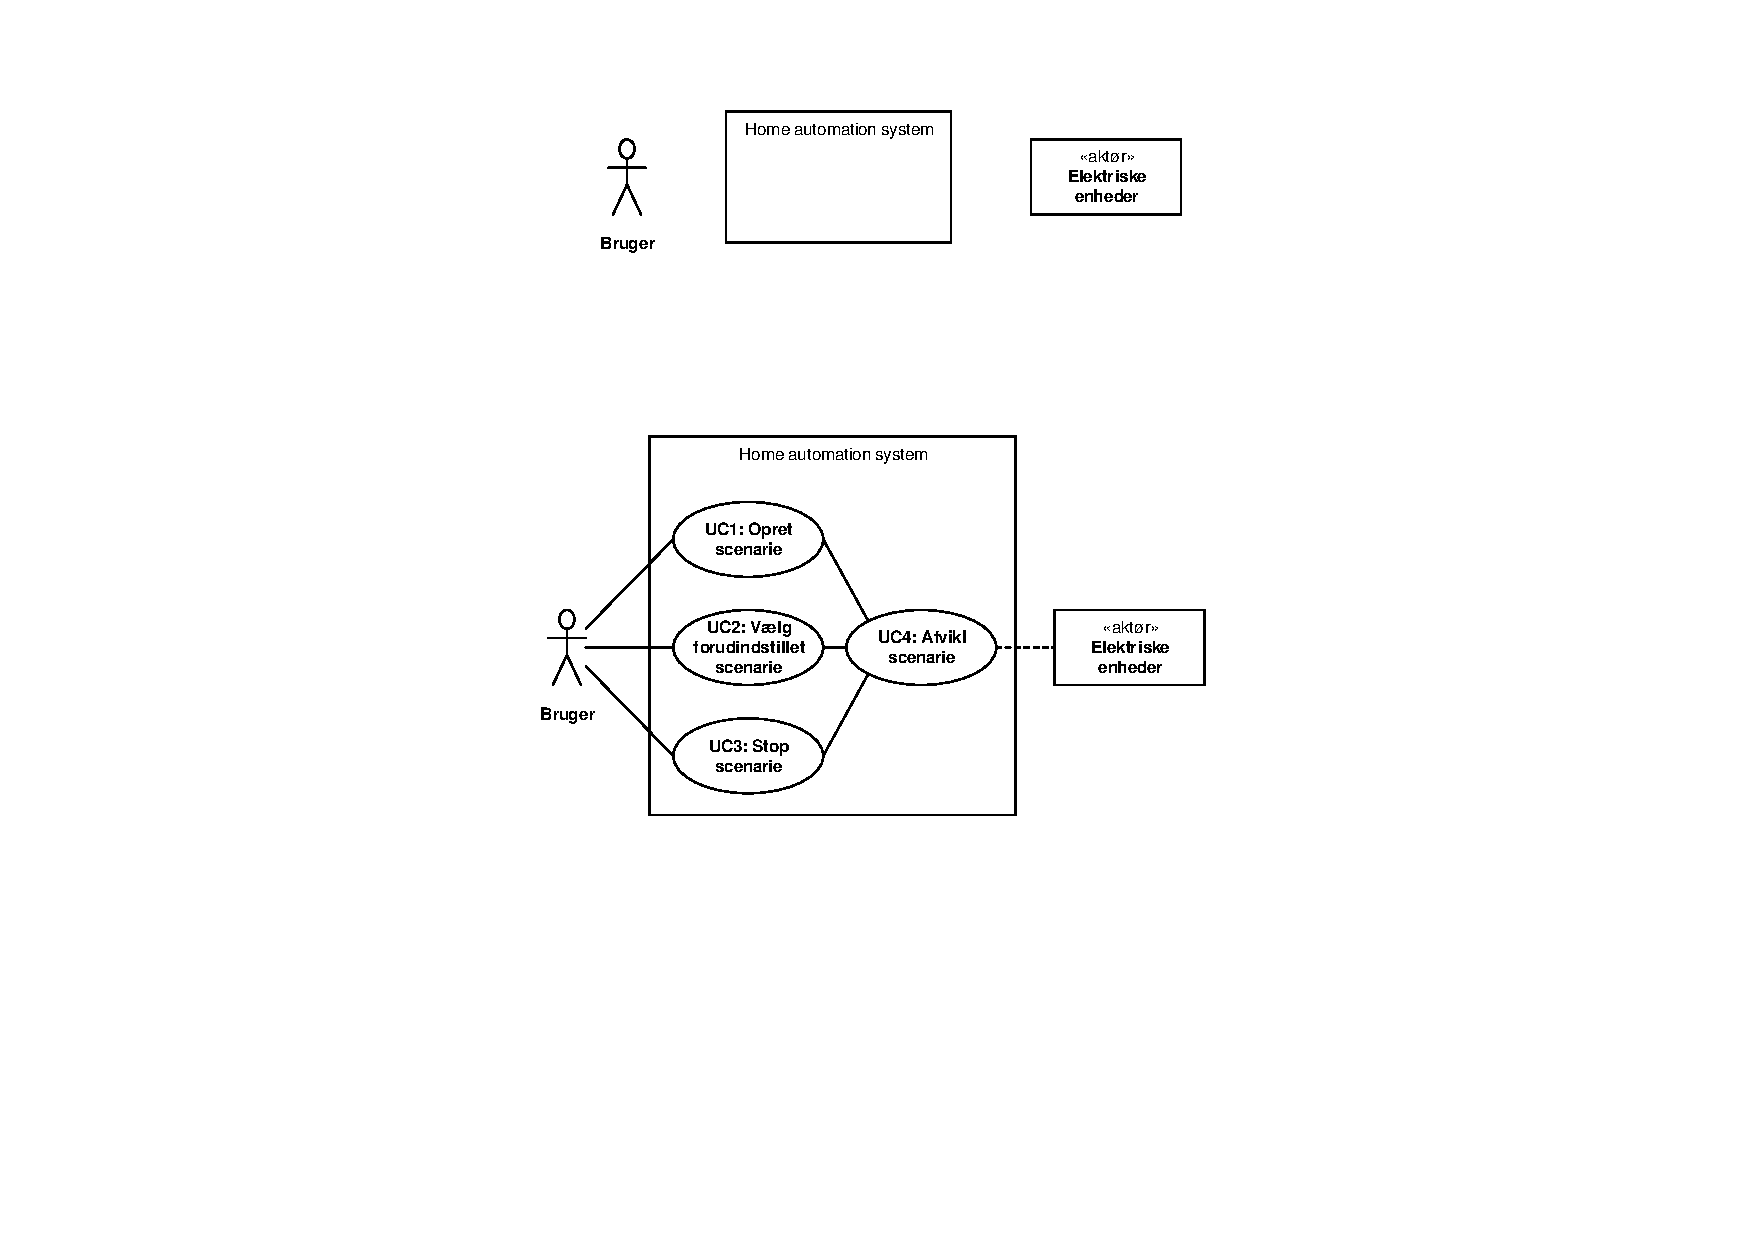
\includegraphics[scale=1,clip=true,trim=220 200 260 209]{../Kravspecifikation/actor.pdf}
\label{fig:uc_diagram}
\caption{Use Case diagram}
\end{figure}

\clearpage

\section{Use Case beskrivelse}
\begin{table}[h]
\begin{tabularx}{\textwidth}{| l | >{\raggedright\arraybackslash}X |} \hline
\textbf{Navn:} 						& UC1: Opret scenarie\\ \hline
\textbf{Mål:}						& Oprette og eksekvere et brugerdefineret scenarie. \\ \hline
\textbf{Initering:}					& Bruger \\ \hline
\textbf{Aktører:} 					& Bruger (primær) \\ \hline
\textbf{Reference:} 					& UC4: Afvikl scenarie \\ \hline
\textbf{Antal samtidige forekomster:} & En \\ \hline
\textbf{Forudsætning:} 				& At de tre koder er indtastet korrekt på kodelåsen, systemet er operationelt og brugeren har valgt "Opret scenarie" i programmet på PC'en.\\ \hline
\textbf{Resultat:}					& Systemet afvikler brugerens scenarie. \\ \hline
\textbf{Hovedscenarie:}				& 

\begin{packed_enum}
\item Systemet præsenterer en liste af aktioner. 
\item Brugeren vælger aktionsnummer. 
	\begin{packed_item}\itemsep1pt \parskip0pt \parsep0pt
	\item {[}Ext 1: Ugyldigt input{]}
	\end{packed_item}
\item Systemet præsenterer en liste af enheder. \label{lasseernice}
\item Brugeren vælger enhed for aktion.
	\begin{packed_item}\itemsep1pt \parskip0pt \parsep0pt
	\item {[}Ext 1: Ugyldigt input{]}
	\end{packed_item}
\item Systemet præsenterer en liste af kommandoer. 
\item Brugeren vælger kommando for aktion. 
	\begin{packed_item}\itemsep1pt \parskip0pt \parsep0pt
	\item {[}Ext 1: Ugyldigt input{]}
	\end{packed_item}
\item Systemet beder om indtastning af et tidspunkt for aktion. 
\item Brugeren indtaster tid for aktion. 
	\begin{packed_item}\itemsep1pt \parskip0pt \parsep0pt
	\item {[}Ext 1: Ugyldigt input{]}
	\end{packed_item}
\item Brugeren præsenteres med listen af aktioner. 
\item Brugeren vælger aktionsnummer (gentag fra punkt \ref{lasseernice}) eller at igangsætte scenariet. 
	\begin{packed_item}\itemsep1pt \parskip0pt \parsep0pt
	\item {[}Ext 1: Ugyldigt input{]}
	\end{packed_item}
\item Programmet sender det konfigurerede scenarie til transmitter-controlleren. 
\item UC4: Afvikl scenarie påbegyndes. 
\item PC-softwaren vender tilbage til hovedmenuen.
\end{packed_enum} \\ \hline
\textbf{Udvidelser:}				&  
\textbf{{[}Ext 1: Ugyldigt input{]}}
	\begin{packed_enum}\itemsep1pt \parskip0pt \parsep0pt
	\item Systemet informerer brugeren om at der er foretaget en forkert indtastning og informerer brugeren om at prøve igen.
	\end{packed_enum}
\\ \hline
\end{tabularx}
\caption{UC1: Opret scenarie}
\label{tbl:UC1}
\end{table}
\clearpage

\begin{table}[h]
\begin{tabularx}{\textwidth}{| l | >{\raggedright\arraybackslash}X |}
\hline
\textbf{Navn:} 						& UC2: Vælg forudindstillet scenarie \\ \hline
\textbf{Mål:}						& Eksekvere et forudindstillet scenarie. \\ \hline
\textbf{Initering:}					& Bruger \\ \hline
\textbf{Aktører:} 					& Bruger (primær) \\ \hline
\textbf{Reference:} 				& UC4: Afvikl scenarie \\ \hline
\textbf{Antal samtidige forekomster:} & En \\ \hline
\textbf{Forudsætning:} 				& At de tre koder er indtastet korrekt på kodelåsen, systemet er operationelt og brugeren har valgt ''Vælg forudindstillet scenarie'' i programmet på PC'en.\\ \hline
\textbf{Resultat:}					& Systemet afvikler brugerens scenarie. \\ \hline
\textbf{Hovedscenarie:}				& 
\begin{packed_enum}\itemsep1pt \parskip0pt \parsep0pt
	\item Systemet præsenterer en liste af scenarier. 
	\item Brugeren vælger scenarie. 
	\begin{packed_item}\itemsep1pt \parskip0pt \parsep0pt
		\item {[}Ext 1: Ugyldigt input{]}
	\end{packed_item}
	\item Programmet sender det konfigurerede scenarie til transmitter-controlleren. 
	\item UC4: Afvikl scenarie påbegyndes. 
	\item PC-softwaren vender tilbage til hovedmenuen.
\end{packed_enum} \\ \hline 
\textbf{Udvidelser:}				& 
\textbf{{[}Ext 1: Ugyldigt input{]}} 
	\begin{packed_enum}\itemsep1pt \parskip0pt \parsep0pt
	\item Systemet informerer brugeren om at der er foretaget en forkert indtastning og informerer brugeren om at prøve igen.
	\item Systemet vender tilbage til hovedscenariet ved forrige punkt.
	\end{packed_enum} \\ \hline
\end{tabularx}
\caption{UC2: Vælg forudindstillet scenarie}
\label{tbl:UC2}
\end{table}
\clearpage

\begin{table}
\begin{tabularx}{\textwidth}{| l | >{\raggedright\arraybackslash}X |}
\hline
\textbf{Navn:} 						& UC3: Stop scenarie \\ \hline
\textbf{Mål:}						& At stoppe al aktivitet på de elektriske enheder. \\ \hline
\textbf{Initering:}					& Bruger \\ \hline
\textbf{Aktører:} 					& Bruger (primær) \\ \hline
\textbf{Reference:} 				& UC4: Afvikl scenarie \\ \hline
\textbf{Antal samtidige forekomster:} & En \\ \hline
\textbf{Forudsætning:} 				& At de tre koder er indtastet korrekt, at systemet er operationelt og at der er et scenarie under afvikling og brugeren har valgt ''Stop scenarie'' i programmet på PC'en.\\ \hline
\textbf{Resultat:}					& Systemet stopper igangværende scenarie. \\ \hline
\textbf{Hovedscenarie:}				& 
\begin{packed_enum}\itemsep1pt \parskip0pt \parsep0pt
	\item Systemet prompter brugeren om vedkommende er sikker.
	\item Brugere vælger "ja".
	\begin{packed_item}\itemsep1pt \parskip0pt \parsep0pt
		\item {[}Ext. 1: Brugeren vælger ''nej''{]}
	\end{packed_item}
	\item UC4: Afvikl scenarie afsluttes.
	\item Der sendes en sluk-kommando til alle enheder.
	\item PC-softwaren vender tilbage til hovedmenuen.
\end{packed_enum} \\ \hline
\textbf{Udvidelser:}				& 
\textbf{{[}Ext 1: Brugeren vælger ''nej''{]}} 
	\begin{packed_enum}\itemsep1pt \parskip0pt \parsep0pt
	\item Systemet vender tilbage til hovedmenuen og UC3: Stop scenarie afsluttes.
	\end{packed_enum} \\ \hline
\end{tabularx}
\caption{UC3: Stop scenarie}
\label{tbl:UC3}
\end{table}
~
\clearpage


\begin{table}
\begin{tabularx}{\textwidth}{| l | >{\raggedright\arraybackslash}X |}
\hline
\textbf{Navn:} 						& UC4: Afvikl scenarie \\ \hline
\textbf{Mål:}						& Afvikler kontinuerligt det valgte scenarie. \\ \hline
\textbf{Initering:}					& UC1 eller UC2 \\ \hline
\textbf{Aktører:} 					& Elektriske enheder (sekundære) \\ \hline
\textbf{Reference:} 				& UC1, UC2 og UC3 \\ \hline
\textbf{Antal samtidige forekomster:} & En \\ \hline
\textbf{Forudsætning:} 				& Systemet er operationelt.\\ \hline
\textbf{Resultat:}					& Systemet afvikler det valgte scenarie. \\ \hline
\textbf{Hovedscenarie:}				& 
\begin{packed_enum}\itemsep1pt \parskip0pt \parsep0pt
	\item Systemet tæller tiden et sekund opad. \label{repeat_UC4}
	\item Systemet tjekker om tiden stemmer overens med en aktion. 
	\item Tiden stemmer ikke overens med en aktion.	
	\begin{packed_item}\itemsep1pt \parskip0pt \parsep0pt
		\item {[}Ext 1: Tiden stemmer overens med en aktion{]}
	\end{packed_item}
	\item Hovedscenariet gentages fra Punkt \ref{repeat_UC4}.
\end{packed_enum} \\ \hline
\textbf{Udvidelser:}				& 
\textbf{{[}Ext 1: Tiden stemmer overens med en aktion{]}} 
	\begin{packed_enum}
		\item Transmitter-controlleren sender den pågældende kommando.
		\item Den pågældende receiver-controller afkoder og udfører den pågældende kommando.
	\end{packed_enum} \\ \hline
\end{tabularx}
\caption{UC4: Afvikl scenarie}
\label{tbl:UC4}
\end{table}
~
\clearpage

\section{Funktionelle Krav} \label{FunkKrav}
Systemet\ldots
\begin{enumerate}\itemsep1pt \parskip0pt \parsep0pt
	\item \ldots \emph{Skal} kunne tænde og slukke for lamper.
	\item \ldots \emph{Skal} kunne dimme op og ned for lamper.
	\item \ldots \emph{Skal} kunne tænde og slukke for et TV.
	\item \ldots \emph{Skal} kunne inkrementere og dekrementere kanal på et TV.
	\item \ldots \emph{Skal} kunne justere volumen op og ned på et TV.
	\item \ldots \emph{Skal} kunne vælge en specifik kanal på et TV.
	\item \ldots \emph{Skal} kunne tænde og slukke for en radio.
	\item \ldots \emph{Skal} kunne søge efter næste eller forrige kanal.
	\item \ldots \emph{Skal} kunne justere volumen op og ned på en radio.
	\item \ldots \emph{Skal} kunne vælge en forudindstillet radiokanal.
	\item \ldots \emph{Må} ikke kunne anvendes uden korrekt kode.
	\item \ldots \emph{Skal} have en GUI.
	\item \ldots \emph{Skal} kunne interageres med via en PC.
	\item \ldots \emph{Skal} give brugeren mulighed for at oprette og eksekvere et scenarie.
	\item \ldots \emph{Skal} give brugeren mulighed for at vælge og eksekvere et forudindstillet scenarie.
	\item \ldots \emph{Skal} give brugeren mulighed for at standse det igangværende scenarie.
	\item \ldots \emph{Skal} kunne håndtere ugyldigt input fra brugeren.
	\item \ldots \emph{Skal} fungere selvom den tilkoblede PC er slukket.
	\item \ldots \emph{Skal} kunne kommunikere med den tilkoblede PC via en seriel forbindelse.
\end{enumerate}

\section{Ikke Funktionelle Krav} \label{ikkeFunkKrav}
Systemet\ldots 
\begin{enumerate}\itemsep1pt \parskip0pt \parsep0pt
	\item \ldots \emph{Skal} fungere på et $18 VAC$ elnet med en frekvens på $50Hz$.
	\item \ldots \emph{Skal} via brugerfladen kunne præsentere en aktionsliste med op til 20 aktioner.
	\item \ldots \emph{Skal} kunne oprette et scenarie med op til 20 aktioner.
	\item \ldots \emph{Skal} kunne afvikle en aktion med en præcision på $\pm 1$ minut, i forhold til den valgte tid.
	\item \ldots \emph{Skal} bruge X.10 protokol\cite{lib:AN236} til kommunikation via elnettet.
	\item \ldots \emph{Skal} kunne afvikle minimum en aktion i minuttet.
	\item \ldots \emph{Skal} rumme 3 predefinerede scenarier.
	\item \ldots \emph{Skal} kunne iværksætte et predefineret scenarie ved højst 5 indtastninger fra brugerens side.
	\item \ldots \emph{Skal} kunne håndtere 2 lamper, et TV og en radio.
	\item \ldots \emph{Skal} via dimmefunktionen i trin af $10\% \pm 1\%$ kunne regulere middelspændingen over en 5mm gul L53-YD LED eller tilsvarende fra $5\%$ til $95\%$ af elnettets spænding.
	\item \ldots \emph{Skal} have en min. up-time på 80\% over en time.
	\item Teksten i UI'en \emph{skal} være grå med hex-farvekode \#C0C0C0 med sort baggrund med hex koden \#000000.
	\item Når en lampe er slukket, \emph{skal} middelstrømmen gennem denne være $0A \pm 50 mA$ over en periode på 10 sekunder.
	\item Transmitter- og reciever-controllererne \emph{skal} være afskærmede af individuelle kasser med dimmensioner på maksimalt $50cm \times 50cm \times 20cm$.
	\item Brugerfladen \emph{skal} være på dansk.
\end{enumerate}
\clearpage
